\title{Homework 2 Report}
\author{
        Hooley Cheng \\
                Department of Mathematics\\
        University of Washington\\
        Seattle, WA, 98105, U.S.
           
}
\date{\today}

\documentclass[12pt]{article}


\usepackage{amsmath}
\usepackage{graphicx}
\usepackage{float}
\usepackage{listings}

\usepackage{titlesec}
\begin{document}
\maketitle

\begin{abstract}
This project intends to investigate various properties of Gabor Filters by serveral differernt examples. We will discuss how the bandwidth affects on the result of Fast-Fourier Transformation of these examples and their spectrograms. Also, we will apply the knowledge into a specific project. 
\end{abstract}

\section{Introduction and Overview}\
	We are going to use a portion of Handel's Messiah as the first example to apply different Gabor Filters: Gaussian Window, Mexican hat wavelet and Shannon Window. During our discussion, we found out a interesting phenomenon that relates our time domain and frequency domain. Later on, after comparing several results, we finally found out that this phenomenon is due to Heisenberg Uncertainty. After that, we take a look into one application example of using the technique to help us reproduce music score.
	
\section{Theoretical Background}
As discussed before, Gaussian Filter is a powerful tool to help us analysis signals when we know the target frequency. However, in some situation, we might want to extract both time and frequency information from our data. Then, directly applying Gaussian Filter and Fourier Transform might not be a good choice. Therefore, we need to establish a new approach that help us to deal with this problem, and we found out that a simple modification of the original filter could help:\\
	\[g_{t,\omega}=e^{i\omega\tau}g(\tau-t)\]
where the new term to the Fourier kernel $g(\tau - t)$ was introduced with the aim of localizing both time and frequency. The Gabor transform, also known as the short-time Fourier transform, is t hen defined as the following:
	\[G[f](t,\omega)=\int_{-\infty}^{\infty}f(\tau)\bar{g}(\tau-t)e^{-i\omega\tau}\]
Thus, the function $g(\tau - t)$ acts as a time filter for localizing the signal over a specific window of time, and we can sliding this window alone the time domain. Also, we found other kernels can also function in a very similar behaviour:
	\[M(t) = (1-t^2)e^{-t^2/2}\]
	which is known as Mexican hat wavelet, and:
	\[ S(t) = \begin{cases} 
      1 & |t - t0|\leq bandwidth \\
      0 & otherwise 
   \end{cases}
\]
which is known as Shannon window.

\section{Algorithm Implementation and Development}
\subsection{Relation between bandwidth and spectrogram}
First, we are going to investigate how the bandwidth affects spectrogram using Gaussian window:

\begin{figure}[H]
\begin{tabular}{cc}
  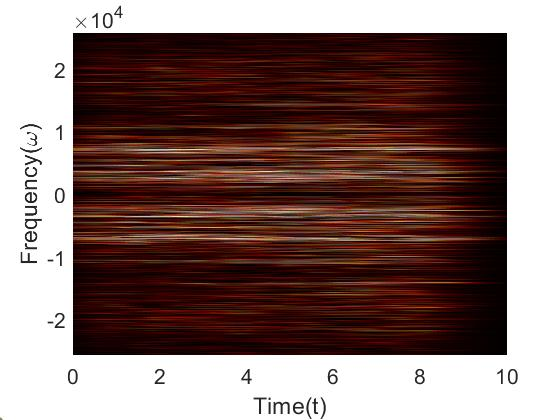
\includegraphics[width=65mm]{s1.jpg} &    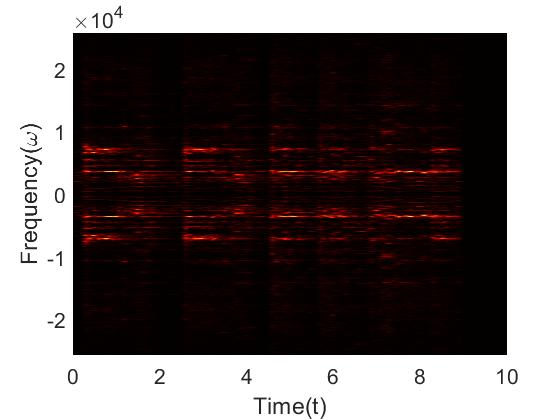
\includegraphics[width=65mm]{s4.jpg} \\
 $a=1$ &  $a=1000$ \\[6pt]\\
\end{tabular}
\end{figure}
Then, we choose another kernel, the Mexican hat wavelet, to compare:
\begin{figure}[H]
\begin{tabular}{cc}
  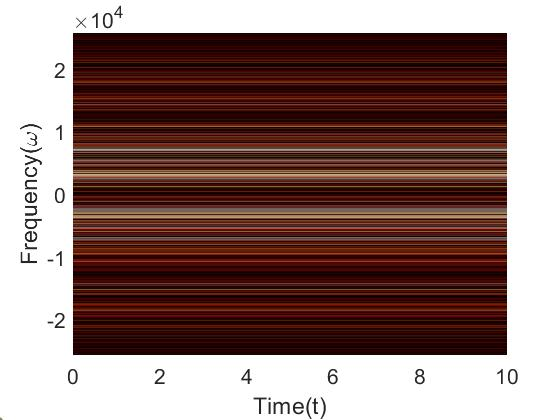
\includegraphics[width=65mm]{m1.jpg} &    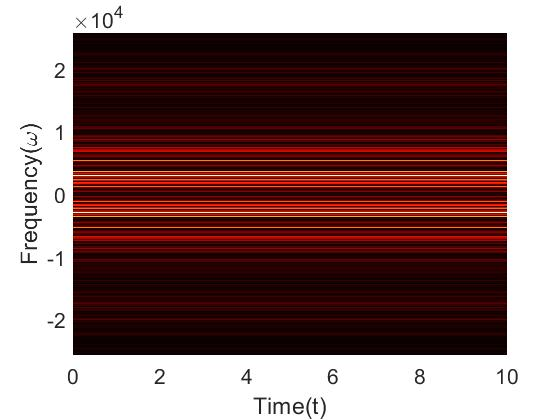
\includegraphics[width=65mm]{m4.jpg} \\
 $a=1$ &  $a=1000$ \\[6pt]\\
\end{tabular}
\end{figure}
and also, we need to try Shannon widow:
\begin{figure}[H]
\begin{tabular}{cc}
  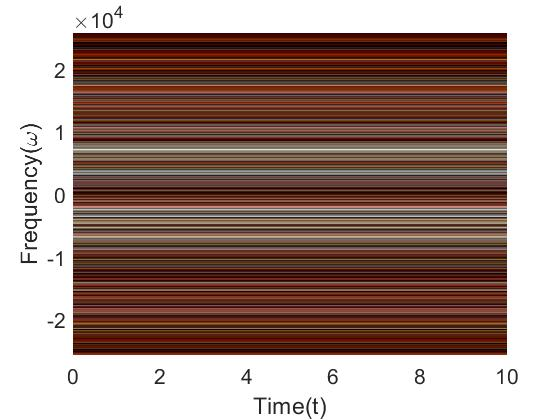
\includegraphics[width=65mm]{h4.jpg} &    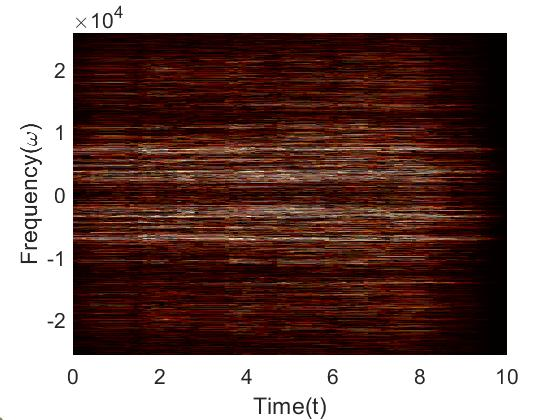
\includegraphics[width=65mm]{h1.jpg} \\
 $1/a \propto 1$ &  $1/a \propto 20$ \\[6pt]\\
\end{tabular}
\end{figure}
We can clearly see the trend from these three examples that as the bandwidth decreasing, the time resolution increases and the frequency resouliton decreases. However, the Mexican hat wavelet seems to have a special property that even though we have narrowed down its band into a very small number, its time resolution is still worse than any other examples.
\subsection{Application of Gabor filtering}
In this section, we going to use Gabor filtering to reproduce the music score of two simple pieces. First, let's take a look at the visualization of the these two pieces:
\begin{figure}[H]
\begin{tabular}{cc}
  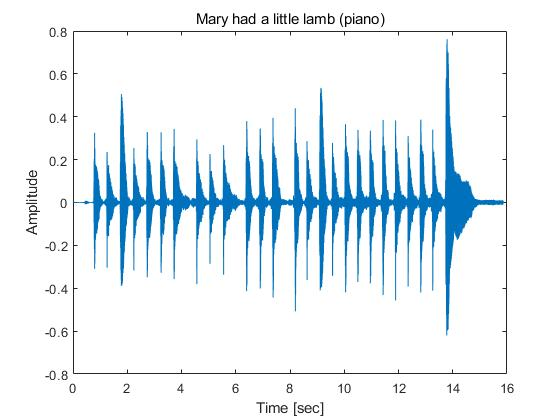
\includegraphics[width=65mm]{p.jpg} &    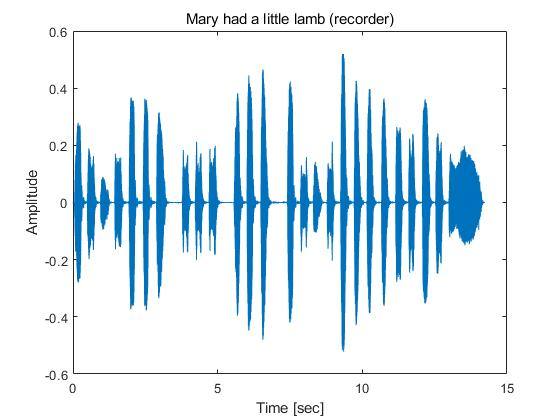
\includegraphics[width=65mm]{r.jpg} \\
\end{tabular}
\end{figure}
From these two graphs, we can see that there are clear gaps between each node. Therefore, if we use proper bandwidth, we can easily seperate them into single node. By setting $a=100$, we can easily extract frequency-time graph of these two pieces:
\begin{figure}[H]
\begin{tabular}{cc}
  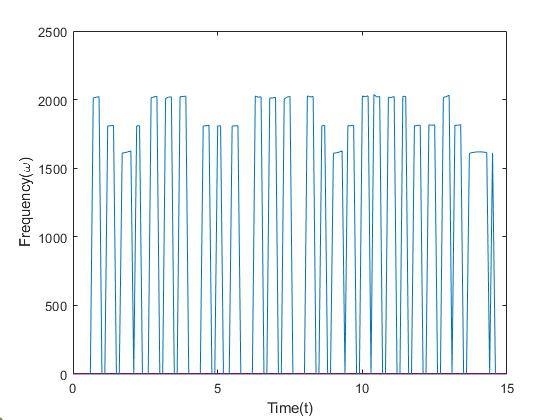
\includegraphics[width=65mm]{pf.jpg} &    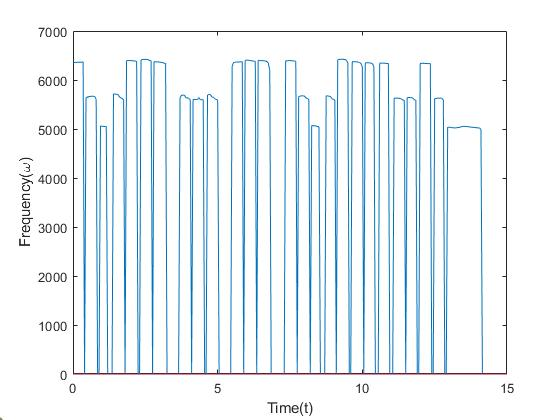
\includegraphics[width=65mm]{rf.jpg} \\
\end{tabular}
\end{figure}
After manually checking the frequency of each node at each time, we can then create a music score graph:
\begin{figure}[H]
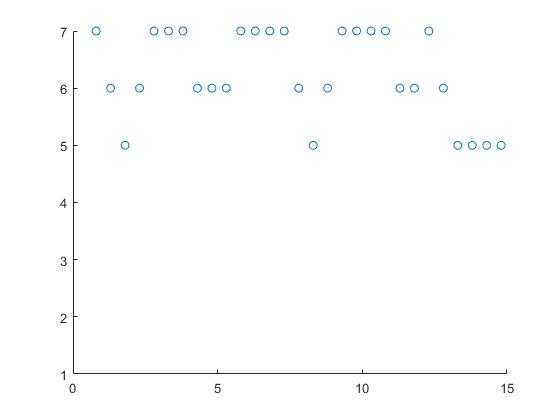
\includegraphics[width=\linewidth]{score.jpg}
\end{figure}
\section{Computational Results}
Here is the time-frequency table of the pieces:
\begin{table}[H]
\begin{tabular}{llllll}
\hline
\multicolumn{1}{|l|}{time(sec)} & \multicolumn{1}{l|}{piano(Hz)} & \multicolumn{1}{l|}{recorder(Hz)} & \multicolumn{1}{l|}{time(sec)} & \multicolumn{1}{l|}{piano(Hz)} & \multicolumn{1}{l|}{recorder(Hz)} \\ \hline
\multicolumn{1}{|l|}{0}         & \multicolumn{1}{l|}{2015}      & \multicolumn{1}{l|}{6362}         & \multicolumn{1}{l|}{7.5}       & \multicolumn{1}{l|}{1614}      & \multicolumn{1}{l|}{5064}         \\ \hline
\multicolumn{1}{|l|}{0.5}       & \multicolumn{1}{l|}{1809}      & \multicolumn{1}{l|}{5668}         & \multicolumn{1}{l|}{8}         & \multicolumn{1}{l|}{1811}      & \multicolumn{1}{l|}{5620}         \\ \hline
\multicolumn{1}{|l|}{1}         & \multicolumn{1}{l|}{1616}      & \multicolumn{1}{l|}{5054}         & \multicolumn{1}{l|}{8.5}       & \multicolumn{1}{l|}{2022}      & \multicolumn{1}{l|}{6422}         \\ \hline
\multicolumn{1}{|l|}{1.5}       & \multicolumn{1}{l|}{1809}      & \multicolumn{1}{l|}{5663}         & \multicolumn{1}{l|}{9}         & \multicolumn{1}{l|}{2021}      & \multicolumn{1}{l|}{6399}         \\ \hline
\multicolumn{1}{|l|}{2}         & \multicolumn{1}{l|}{2017}      & \multicolumn{1}{l|}{6397}         & \multicolumn{1}{l|}{9.5}       & \multicolumn{1}{l|}{2019}      & \multicolumn{1}{l|}{6349}         \\ \hline
\multicolumn{1}{|l|}{2.5}       & \multicolumn{1}{l|}{2015}      & \multicolumn{1}{l|}{6421}         & \multicolumn{1}{l|}{10}        & \multicolumn{1}{l|}{2021}      & \multicolumn{1}{l|}{6344}         \\ \hline
\multicolumn{1}{|l|}{3}         & \multicolumn{1}{l|}{2023}      & \multicolumn{1}{l|}{6369}         & \multicolumn{1}{l|}{10.5}      & \multicolumn{1}{l|}{1812}      & \multicolumn{1}{l|}{5623}         \\ \hline
\multicolumn{1}{|l|}{3.5}       & \multicolumn{1}{l|}{1810}      & \multicolumn{1}{l|}{5636}         & \multicolumn{1}{l|}{11}        & \multicolumn{1}{l|}{1812}      & \multicolumn{1}{l|}{5629}         \\ \hline
\multicolumn{1}{|l|}{4}         & \multicolumn{1}{l|}{1808}      & \multicolumn{1}{l|}{5599}         & \multicolumn{1}{l|}{11.5}      & \multicolumn{1}{l|}{2019}      & \multicolumn{1}{l|}{6339}         \\ \hline
\multicolumn{1}{|l|}{4.5}       & \multicolumn{1}{l|}{1809}      & \multicolumn{1}{l|}{5614}         & \multicolumn{1}{l|}{12}        & \multicolumn{1}{l|}{1811}      & \multicolumn{1}{l|}{5630}         \\ \hline
\multicolumn{1}{|l|}{5}         & \multicolumn{1}{l|}{2019}      & \multicolumn{1}{l|}{6368}         & \multicolumn{1}{l|}{12.5}      & \multicolumn{1}{l|}{1611}      & \multicolumn{1}{l|}{5033}         \\ \hline
\multicolumn{1}{|l|}{5.5}       & \multicolumn{1}{l|}{2015}      & \multicolumn{1}{l|}{6395}         & \multicolumn{1}{l|}{13}        & \multicolumn{1}{l|}{1620}      & \multicolumn{1}{l|}{5034}         \\ \hline
\multicolumn{1}{|l|}{6}         & \multicolumn{1}{l|}{2021}      & \multicolumn{1}{l|}{6392}         & \multicolumn{1}{l|}{13.5}      & \multicolumn{1}{l|}{1613}      & \multicolumn{1}{l|}{5046}         \\ \hline
\multicolumn{1}{|l|}{6.5}       & \multicolumn{1}{l|}{2019}      & \multicolumn{1}{l|}{6396}         & \multicolumn{1}{l|}{14}        & \multicolumn{1}{l|}{1619}      & \multicolumn{1}{l|}{5023}         \\ \hline
\multicolumn{1}{|l|}{7}         & \multicolumn{1}{l|}{1810}      & \multicolumn{1}{l|}{5676}         & \multicolumn{1}{l|}{}          & \multicolumn{1}{l|}{}          & \multicolumn{1}{l|}{}             \\ \hline
                                &                                &                                   &                                &                                &                                   \\

\end{tabular}
\end{table}
\section{Summary and Conclusions}
Due to the Heisenberg Uncertainty, It is impossible to get accurate information on both time domain and frequency domain, and that is the reason behinds the phenomenon that we found out during 3.1 section. As getting more accurate in time, we increased our time resolution while decreasing the frequency resolution.

\section{Appendix A}
Y = fftn(X) returns the multidimensional Fourier transform of an N-D array using a fast Fourier transform algorithm. The N-D transform is equivalent to computing the 1-D transform along each dimension of X. The output Y is the same size as X.\\

X = ifftn(Y) returns the multidimensional discrete inverse Fourier transform of an N-D array using a fast Fourier transform algorithm. The N-D inverse transform is equivalent to computing the 1-D inverse transform along each dimension of Y. The output X is the same size as Y.\\

Y = fftshift(X) rearranges a Fourier transform X by shifting the zero-frequency component to the center of the array.
If X is a vector, then fftshift swaps the left and right halves of X.
If X is a matrix, then fftshift swaps the first quadrant of X with the third, and the second quadrant with the fourth.
If X is a multidimensional array, then fftshift swaps half-spaces of X along each dimension.\\

X = ifftshift(Y) rearranges a zero-frequency-shifted Fourier transform Y back to the original transform output. In other words, ifftshift undoes the result of fftshift.
If Y is a vector, then ifftshift swaps the left and right halves of Y.
If Y is a matrix, then ifftshift swaps the first quadrant of Y with the third, and the second quadrant with the fourth.
If Y is a multidimensional array, then ifftshift swaps half-spaces of Y along each dimension.\\
\section{Appendix B: Matlab Source Code}
\begin{lstlisting}[caption={Generating Spectrogram of Gaussian Kernel}, frame=single]
load handel
S = y';
n = length(S);
t2 = (1:length(S))/Fs;
t = t2(1:n); 
L = t(end);
k=(2*pi/L)*[0:n/2 -n/2:-1]; 
ks=fftshift(k);
tau = 3;
a = 1000;
figure(2)
tslide=0:0.1:10;
Sgt_spec = zeros(length(tslide),n);
for j=1:length(tslide)
    g=exp(-a*(t-tslide(j)).^2); 
    Sg=g.*S; 
    Sgt=fft(Sg); 
    Sgt_spec(j,:) = fftshift(abs(Sgt));
end
pcolor(tslide,ks,Sgt_spec.'), 
shading interp 
set(gca,'Fontsize',16) 
colormap(hot)
xlabel('Time(t)')
ylabel('Frequency(\omega)') 
\end{lstlisting}

\begin{lstlisting}[caption={Generating Spectrogram of Mexican Hat Wavelet}, frame=single]
a=10;
figure(2)
tslide=0:0.1:10;
Sgt_spec = zeros(length(tslide),n);
for j=1:length(tslide)
    mex = (1-a.*(t-t0).^2).*exp(-a.*(t-t0).^2);
    Sg=mex.*S; 
    Sgt=fft(Sg); 
    Sgt_spec(j,:) = fftshift(abs(Sgt)); 
end
pcolor(tslide,ks,Sgt_spec.'), 
shading interp 
set(gca,'Fontsize',16) 
colormap(hot)
xlabel('Time(t)')
ylabel('Frequency(\omega)')
\end{lstlisting}

\begin{lstlisting}[caption={Generating Spectrogram of Shannon Window}, frame=single]
a=1;
figure(2)
tslide=0:0.1:10;
Sgt_spec = zeros(length(tslide),n);
for j=1:length(tslide)
    t0 = tslide(j);
    y = abs(t-tslide(j))<=a;
    Sg=y.*S; 
    Sgt=fft(Sg); 
    Sgt_spec(j,:) = fftshift(abs(Sgt)); 
end
pcolor(tslide,ks,Sgt_spec.'), 
shading interp 
set(gca,'Fontsize',16) 
colormap(hot)
xlabel('Time(t)')
ylabel('Frequency(\omega)')
\end{lstlisting}

\begin{lstlisting}[caption={Generating Frequency-Time graph of music piece}, frame=single]
figure(9)
[y,Fs] = audioread('music2.wav');
tr_rec=length(y)/Fs; % record time in seconds
plot((1:length(y))/Fs,y);
xlabel('Time [sec]'); ylabel('Amplitude');
title('Mary had a little lamb (recorder)');

a = 100;
tslide=0:0.05:15;
S = y';
n = length(S);
t2 = (1:length(S))/Fs;
t = t2(1:n); 
L = t(end);
k=(2*pi/L)*[0:n/2-1 -n/2:-1]; 
ks=fftshift(k);

score = zeros(length(tslide));
for j=1:length(tslide)
    t0 = tslide(j);
    g=exp(-a*(t-tslide(j)).^2);  
    Sg=g.*S; 
    Sgt=fft(Sg); 
    y = Sg(find(Sg==max(Sg)));
    if y >=0.05
        x = k(find(Sgt==max(Sgt)));
        score(j) = abs(x);
    end

end
figure(9)
plot(tslide, score);
xlabel('Time(t)')
ylabel('Frequency(\omega)')
\end{lstlisting}
\end{document}